\documentclass[9pt]{beamer}
\mode<presentation>{}
\setbeamertemplate{itemize items}[default]
\usepackage{graphicx}
\usepackage{amsmath}
\usepackage{amssymb}
\usepackage{mathtools}
\usepackage{physics}
\usepackage{commath}
\usepackage{setspace}
\usepackage{float}

\setbeamercovered{transparent}


\DeclarePairedDelimiterX{\inp}[2]{\langle}{\rangle}{#1, #2}

\newcommand{\R}{\mathbb{R}}
\newcommand{\F}{\mathbb{F}}
\newcommand{\C}{\mathbb{C}}
\newcommand{\V}{\mathcal{V}}
\newcommand{\bx}{\mathbf{x}}


\subtitle{Multi-Agent Area Coverage Control Using Reinforcement Learning}
\author{Adekunle Adepegba, Suruz Miah, Davide Spinello \\
Summarized by Simon Hu}
\date{\today}
\usetheme{Berlin}
\usefonttheme{professionalfonts}

\begin{document}
	
\begin{frame}
\titlepage
\end{frame}
	
\begin{frame}{Outline}
\tableofcontents
\end{frame}

\section{Introduction}
\begin{frame}{Problem Statement}
	\begin{itemize}
		\item Given a group of $N$ homogeneous agents moving in an environment $\Omega \subset \R^2$, find a configuration $p = (p_1, p_2, \dots, p_N) \in \R^{2^N}$ of these agents that maximizes 
		\begin{equation}
			\displaystyle \mathcal{H}(p,t) = \int_{\Omega}{\max\limits_{i=1, 2, \dots, N}{f_i(\:\norm{q - p_i})} \phi(q, t) \: \dif q}.
		\end{equation}
		\item $f_i : \Omega \to \R_{\geq 0}$ is Lesbegue measurable, non-increasing, and is a function of the distance between $p_i$ and $q$. We will consider $f(x) = -x^2$. 
		\item $\phi : \Omega \times \R_{\geq 0} \to \R_{\geq 0}$ is the \textit{risk density}. It measures our belief in an event happening at point $q$ at time $t$. 
		\item Applications: harbor patrol, search and rescue operations, ocean data collection. 
	\end{itemize}
\end{frame}

\begin{frame}{Voronoi Tesselations}
	\begin{itemize}
		\item A collection $S = (S_1, S_2, \dots, S_M)$ is a partition of $\Omega$ if each pair of $S_i$ have disjoint interior and their union is $\Omega$. 
		\item The Voronoi partition is a particular partition given by $\V = (\V_1, \V_2, \dots, \V_L)$ where
		\begin{equation*}
			\displaystyle \V_i = \left\{ q \in \Omega \: | \: \norm{q - p_i} \leq \norm{q - p_j}, \forall j \neq i \right\}.
		\end{equation*}  
		\item $c_{\V_i}$ and $m_{\V_i}$ are the centroid and mass of the $i$-th cell. 
	\end{itemize}
	\begin{figure}[H]
		\centering 
		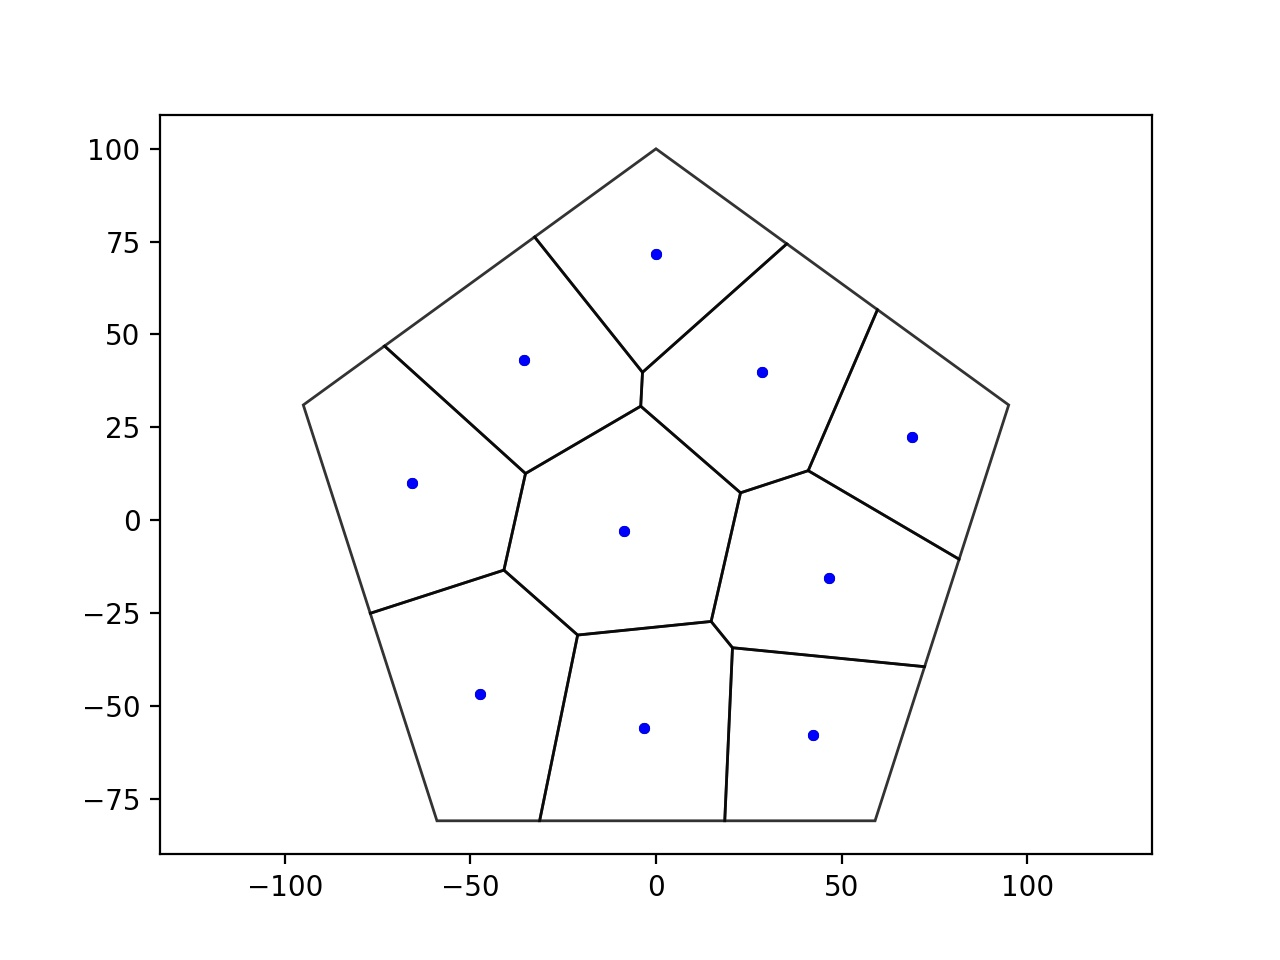
\includegraphics[scale=0.33]{voronoi_partition}
	\end{figure}
\end{frame}

\begin{frame}{Voronoi Tesselations}
	\begin{itemize}
		\item If we partition $\Omega$ according to $\V$ we can rewrite the cost as 
		\begin{equation*}
			\displaystyle \mathcal{H}(p, t) = \sum\limits_{i=1}^{N}{\int_{\V_i}{f_i(\:\norm{q - p_i}) \phi(q,t)\: \dif q}}.
		\end{equation*}
		\item Each agent only needs information from its \textit{neighbors} to compute its contribution to the global cost. Any algorithm taking advantage of this is \textit{spatially distributed}. 
	\end{itemize}
\end{frame}

\section{Optimal Strategy}
\begin{frame}{Optimal Strategy}
	\begin{itemize}
		\item (Cort\'es et al. 2004). The control strategy where each agent moves towards the centroid of its Voronoi cell locally solves the area coverage control problem. 
	\end{itemize}
	\begin{figure}[H]
		\centering 
		\includegraphics[scale=0.4]{minimum_energy_voronoi}
	\end{figure}
\end{frame}

\section{Reinforcement Learning Solution}
\begin{frame}{Reinforcement Learning Approach}
	\begin{itemize}
		\item Let $e_i = c_{\V_i} - p_i$. The authors consider the value function 
		\begin{equation*}
			\displaystyle V(e_i) = \sum\limits_{\kappa = k}^{\infty}{e_i^TQe_i + u_i^TRu_i}
		\end{equation*}
		where $Q, R \in \R^{2 \times 2}$ are positive definite.
		\item Perform the standard trick to write this as the HBJ 
		\begin{equation*}
			\displaystyle V^*(e_i) = \min\limits_{u_i}{\left[ e_i^TQe_i + u_i^TRu_i+ V^{next}(e_i) \right]}.
		\end{equation*} 
		\item Now we approximate the Value function $V(e_i)$ and policy $u_i$ as neural networks.  
	\end{itemize}
\end{frame}
\begin{frame}{Soft Actor-Critic Method}
	\begin{itemize}
		\item The authors basically use the SAC DDPG algorithm we implemented in homework 4, with slight modifications.
		\begin{itemize}
			\item They use least-squares loss instead of MSE. 
			\item Soft updates don't use the update rule 
				\begin{equation}
					\label{soft update}
					w_{target} \leftarrow \alpha w_{target} + (1 - \alpha) w_{source} 
				\end{equation}
				but use the weights from the policy networks to update the weights from the Value function network. 
		\end{itemize}
		\item Since they use least-squares loss, they actually compute the analytical form, which involves taking inverses.
		\item We will use the update rule (\ref{soft update}), use MSE loss, and actually implement the network.
	\end{itemize}
\end{frame}
\section{Simulation Results}
\begin{frame}
	\begin{figure}[H]
		\centering 
		\includegraphics[scale=0.2]{config}
		\includegraphics[scale=0.2]{coverage}
	\end{figure}
	\begin{figure}[H]
		\centering 
		\includegraphics[scale=0.2]{error}
		\centering 
		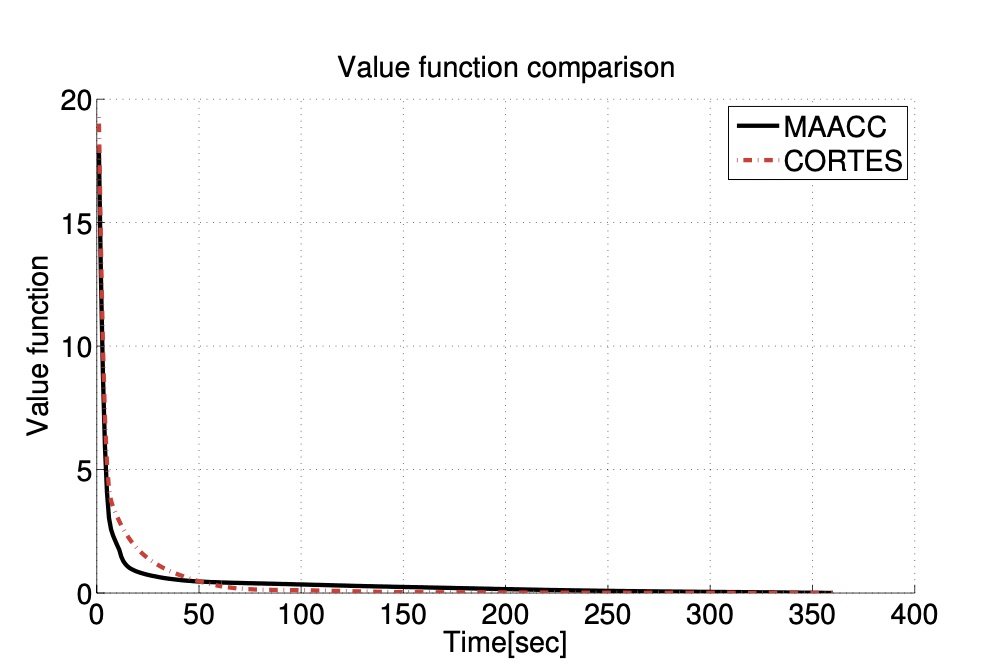
\includegraphics[scale=0.2]{value}
	\end{figure}
\end{frame}

\section{Conclusion}
\begin{frame}{Good, Bad, and the Ugly}
	\begin{itemize}
		\item Good:
		\begin{itemize}
			\item RL methods are robust to changes in the environment. In many applications your environment is dynamic. 
			\item PD Feedback Controllers are OK for handling changes but may not be good at learning the dynamics of the environment. 
		\end{itemize}
		\item Bad:
		\begin{itemize}
			\item You can just implement a really finely tuned PD controller to solve this problem.
		\end{itemize}
		\item Ugly:
		\begin{itemize}
			\item Each agent keeps track of its OWN target and source, actor and critic networks. This is not very scalable!  
		\end{itemize}
	\end{itemize}
\end{frame}

\end{document}